\documentclass[12pt,letterpaper,fleqn]{article}

% Page layout
\usepackage[margin=1in]{geometry}
\usepackage{setspace}
\onehalfspacing

% Math packages
\usepackage{amsmath,amssymb}

% Figures and tables
\usepackage{graphicx}
\usepackage{booktabs}
\usepackage{subcaption}


\usepackage{titlesec}

\titlespacing*{\section}{0pt}{0.8ex}{0.3ex}
\titlespacing*{\subsection}{0pt}{0.6ex}{0.2ex}
\titlespacing*{\subsubsection}{0pt}{0.5ex}{0.15ex}


% Citations
\usepackage[american]{babel}
\usepackage{csquotes}
\usepackage[
style=apa,
backend=biber,
sorting=nyt
]{biblatex}
\addbibresource{references.bib}

% Hyperlinks
\usepackage{hyperref}

% Left aligned equations (fleqn)
\setlength{\mathindent}{0pt}

% Custom commands
\newcommand{\E}{\mathbb{E}}
\newcommand{\Var}{\mathrm{Var}}
\newcommand{\Cov}{\mathrm{Cov}}
\newcommand{\Corr}{\mathrm{Corr}}
\newcommand{\Prb}{\mathrm{Pr}}

%------------------------------------------------
% Title block
%------------------------------------------------

\title{\large\bfseries
Explore the Best Bayesian Model for Dynamic Emotional Network
}

\author{
\small
Marc Shi,  Yu Chang \\
 \small
The University of British Columbia
}

\date{\small
STAT 405: Bayesian Statistics \\
Instructor: Dr.~Alexandre Bouchard-Côté \\
April 2026 \\
\href{https://github.com/Marclianjie/STAT405-Project-}{GitHub Repo}
}

%------------------------------------------------

\begin{document}


\maketitle

\section{Literature Review}

Emotions play a fundamental role in psychological well-being and daily functioning, and understanding how emotional states evolve over time has become an important topic in psychology and behavioral science. Traditional research on affect has focused on static summaries of emotion, such as average levels of positive or negative affect measured through questionnaires. However, such approaches ignore the temporal dynamics of emotional experiences. Emotional states fluctuate continuously and are influenced by both internal processes and external factors, motivating recent research that models emotional experiences as dynamic systems in which emotions at one moment may influence emotions at later moments.

Despite its strengths, this modeling approach implicitly assumes that the observed emotion scores directly represent the true emotional state of an individual. From a statistical perspective, this assumption can be viewed as naive because psychological measurements are often subject to measurement error. Self-reported emotion ratings may reflect not only the true emotional state but also random reporting noise. As a result, a natural Bayesian alternative is to introduce a latent-state formulation, in which the true emotional state is treated as an unobserved variable and the reported emotion scores are viewed as noisy observations generated from a likelihood distribution conditional on the underlying emotional state. This perspective allows the model to explicitly account for measurement error.

In this project, we adopt such a Bayesian framework to study emotional dynamics using the ESM dataset. We consider three models. The first is a naive Bayesian model that assumes the latent emotional states are independent across time. The second is a Hidden Markov Model (HMM), in which the latent emotional state evolves according to a Markov transition process over time. The third is an HMM with exogenous factors, where additional external variables influence the current emotional state. By comparing these models, we aim to investigate whether incorporating temporal dependence and exogenous variables improves predictive performance and provides a better explanation of the observed emotional measurements through the generative model.

In addition to comparing modeling approaches, we also investigate different algorithms for approximating the posterior distribution. Specifically, we compare two Bayesian inference methods: Hamiltonian Monte Carlo (HMC) and Variational Inference (VI). By applying both algorithms to our Hidden Markov Model, we aim to examine the trade-off between computational efficiency and posterior accuracy in modeling emotional dynamics.



\section{Exploratory Data Analysis}

\subsection{Choosing the Initial Focal Emotion}

Before fitting the Bayesian models, we carried out a brief exploratory screening analysis to identify a reasonable initial emotion for the univariate naive model. We used a two-step procedure.

First, we examined the Spearman correlation heatmap for the nine emotion variables (Figure~\ref{fig:corr_heatmap}). The heatmap showed that \texttt{happy} was strongly associated with several other positive emotions, especially \texttt{pleased} and \texttt{enthusiastic}, while also showing moderate negative association with several negative emotions. This suggested that \texttt{happy} may occupy a relatively central position in the emotion system.

Second, because correlation alone does not fully capture predictive ability, we performed a one-step-ahead screening analysis using leave-one-subject-out cross-validation. See Table~\ref{tab:overall_scores} of the resulting ranking in the appendix for a more detailed explanation. Under this criterion, \texttt{happy} ranked first, with the largest mean relative reduction in prediction error. Since \texttt{happy} was supported by both the correlation-based and predictive screening analyses, we selected it as the focal emotion for the univariate naive Bayesian model.

\subsection{Temporal Dependence of Happy}

To examine whether \texttt{happy} exhibits temporal dependence, we first considered the autocorrelation function (ACF) of the average \texttt{happy} series over the ordered day-by-beep index. As shown in Figure~\ref{fig:happy_acf_ccf_combined}, the lag-1 autocorrelation is relatively weak, but there are clear positive spikes at lags 5, 10, and 15. Since the data contain five beeps per day, these peaks suggest a recurring day-level pattern in \texttt{happy} rather than a purely independent sequence. This provides empirical support for modelling temporal dependence instead of assuming an i.i.d.\ structure.

We then examined the cross-correlation function (CCF) between \texttt{happy} and two closely related positive emotions, \texttt{pleased} and \texttt{enthusiastic}. Figure~\ref{fig:happy_acf_ccf_combined} shows that both pairs display their strongest positive association near lag 0, indicating that these emotions tend to move together contemporaneously. The relationship between \texttt{happy} and \texttt{pleased} is especially strong, while the \texttt{happy}--\texttt{enthusiastic} association is somewhat weaker but still clearly positive around zero lag. In addition, several smaller peaks appear at multiples of 5, suggesting that these positive emotions may share a similar daily rhythm. Overall, these plots indicate that \texttt{happy} is temporally structured and closely connected to other positive emotions, which supports the use of time-dependent latent-state models.


\begin{figure}[htbp]
    \centering
    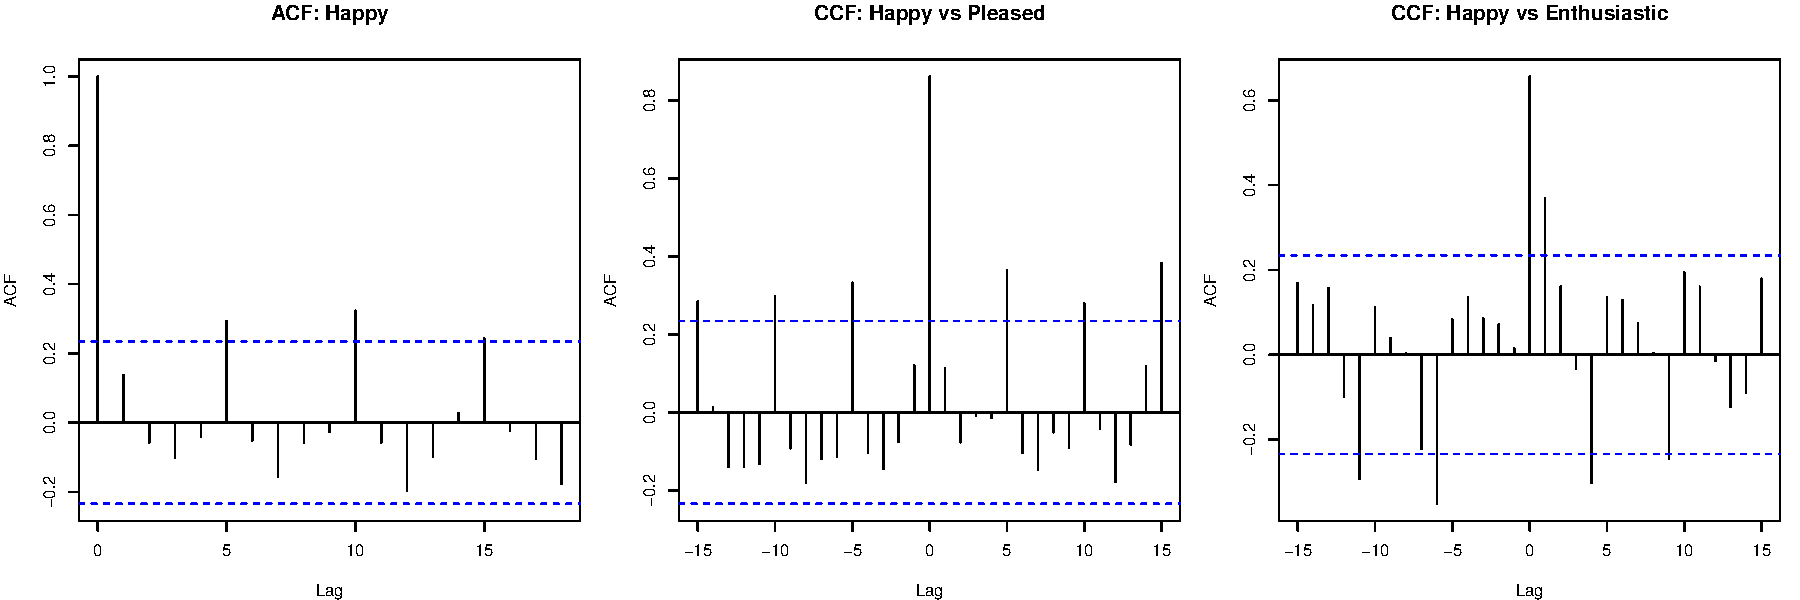
\includegraphics[width=\textwidth]{happy_acf_ccf_combined.pdf}
    \caption{Autocorrelation of \texttt{happy} and cross-correlations of \texttt{happy} with \texttt{pleased} and \texttt{enthusiastic}.}
    \label{fig:happy_acf_ccf_combined}
\end{figure}


\section{Methodology}
\subsection{Models}
\subsubsection{Naive Model}

As a baseline, we use an independent latent-variable model with an ordered logistic likelihood. For each observation \(i=1,\dots,N\), let \(y_i \in \{1,2,3,4,5,6,7\}\) denote the observed ordinal happiness rating and let \(x_i \in \mathbb{R}\) denote a latent continuous happiness level. We assume
\[
x_i \overset{\mathrm{iid}}{\sim} \mathcal{N}(\mu,\sigma^2),
\qquad
\mu \sim \mathcal{N}(0,1.5^2),
\qquad
\sigma \sim \mathrm{Exponential}(1).
\]
Conditional on \(x_i\), the response follows an ordered logistic model,
\[
y_i \mid x_i \sim \mathrm{OrderedLogistic}(x_i,\mathbf{c}),
\]
where the cutpoints are fixed at
\[
\mathbf{c}=(-2.5,-1.5,-0.5,0.5,1.5,2.5).
\]
These cutpoints place \(0\) at the center of the latent scale, corresponding to the middle of the 7-point response scale. Equivalently, the model can be written using a latent logistic noise term:
\[
y_i =
\begin{cases}
1, & x_i+\epsilon_i \le c_1,\\
2, & c_1 < x_i+\epsilon_i \le c_2,\\
\vdots \\
7, & x_i+\epsilon_i > c_6,
\end{cases}
\qquad
\epsilon_i \sim \mathrm{Logistic}(0,1).
\]
This naive model ignores temporal dependence, subject-specific dynamics, and cross-emotion effects, and instead treats all observations as exchangeable draws from a common latent distribution.

\subsubsection{Intermediate Model (with Time Structure)}

We next extend the naive model by allowing the latent happiness process to evolve over time. Let \(x_i\) again denote the latent continuous happiness state at observation \(i\). For observations with available lagged values, we assume
\[
x_i \mid x_{i-1},x_{i-5} \sim \mathcal{N}(\mu_i,\sigma^2),
\]
with conditional mean
\[
\mu_i = \alpha + \beta_1 x_{i-1} + \beta_5 x_{i-5}.
\]
Thus, the current latent happiness level depends on both the immediately previous latent state and the latent state five prompts earlier. For early observations where the required lags are unavailable, the latent state is initialized from the baseline level:
\[
x_i \sim \mathcal{N}(\alpha,\sigma^2).
\]
We place priors
\[
\alpha \sim \mathcal{N}(0,1.5^2), \qquad
\beta_1 \sim \mathcal{N}(0,1), \qquad
\beta_5 \sim \mathcal{N}(0,1), \qquad
\sigma \sim \mathrm{Exponential}(1).
\]
The observation model remains the same as in the naive model.
Unlike the naive model, this specification preserves the ordinal likelihood while introducing temporal dependence in the latent process. Missing observed happiness ratings are not removed from the time series; instead, the latent process is defined over all time points and the likelihood is applied only to observed responses, thereby preserving the lag structure.

\subsubsection{Extended Model (with Time Structure and Additional Predictors)}

Finally, we consider an extension of the intermediate model that incorporates additional lagged emotion predictors. Based on the exploratory screening analysis, the selected predictors were \texttt{enthusiastic}, \texttt{pleased}, and \texttt{relaxed}. Let
\[
e_{i-1}, \quad p_{i-1}, \quad r_{i-1}
\]
denote the lagged values of these three predictors at the previous prompt. We then model the latent happiness state as
\[
x_i \mid x_{i-1},x_{i-5},e_{i-1},p_{i-1},r_{i-1}
\sim \mathcal{N}(\mu_i,\sigma^2),
\]
where
\[
\mu_i
=
\alpha
+\beta_1 x_{i-1}
+\beta_5 x_{i-5}
+\gamma_1 e_{i-1}
+\gamma_2 p_{i-1}
+\gamma_3 r_{i-1}.
\]
Here, \(\beta_1\) and \(\beta_5\) capture autoregressive dependence in latent happiness, while \(\gamma_1,\gamma_2,\gamma_3\) measure the contributions of lagged enthusiasm, pleased, and relaxed scores, respectively. For observations where lagged values are unavailable, the latent state is again initialized from
\[
x_i \sim \mathcal{N}(\alpha,\sigma^2).
\]
We place priors
\[
\alpha \sim \mathcal{N}(0,1.5^2), \qquad
\beta_1 \sim \mathcal{N}(0,1), \qquad
\beta_5 \sim \mathcal{N}(0,1),
\]
\[
\gamma_1 \sim \mathcal{N}(0,1), \qquad
\gamma_2 \sim \mathcal{N}(0,1), \qquad
\gamma_3 \sim \mathcal{N}(0,1), \qquad
\sigma \sim \mathrm{Exponential}(1).
\]
The observation model remains the same as in the previous models.
This model allows future happiness ratings to be explained jointly by persistence in the latent happiness process and by lagged values of related positive-emotion variables.
\subsection{Posterior Computation Methods}

For each of the three models described above, posterior inference is carried out using two complementary approaches implemented in \texttt{Stan}: Hamiltonian Monte Carlo (HMC) and Variational Inference (VI).

The primary method is Hamiltonian Monte Carlo, specifically the No-U-Turn Sampler (NUTS), which is used to generate samples from the exact posterior distribution up to Monte Carlo error. In addition, we employ variational inference as an approximate alternative. Variational inference reframes posterior computation as an optimization problem by approximating the true posterior distribution with a member of a predefined family of distributions. In this study, we use the mean-field variational family, which assumes independence among all parameters and latent variables. While this assumption enables substantial computational gains, it may lead to underestimation of posterior uncertainty and reduced accuracy when strong dependencies are present.

To facilitate a direct comparison between the two approaches, we draw \(3000\) posterior samples from both methods. For HMC, these correspond to Monte Carlo samples obtained after warmup, while for variational inference, they are samples drawn from the optimized variational approximation. This allows for consistent evaluation of posterior summaries and predictive performance across methods.



\section{Model and Posterior Comparison Results}

To compare both model performance and the accuracy of posterior approximation methods, we evaluate predictive performance using approximate leave-one-out cross-validation (LOO), implemented via the \texttt{loo} package. This approach provides a principled, data-efficient measure of out-of-sample predictive ability without requiring an explicit train–test split.

LOO estimates the expected log predictive density (ELPD), defined as
\[
\mathrm{ELPD} = \sum_{i=1}^N \log p(y_i \mid y_{-i}),
\]
where \(y_{-i}\) denotes the dataset with the \(i\)-th observation removed. Intuitively, ELPD measures how well a model predicts each observation when that observation is not used for fitting. Larger values of ELPD indicate better predictive performance.

In practice, exact leave-one-out cross-validation is computationally expensive. The \texttt{loo} package uses Pareto-smoothed importance sampling (PSIS) to approximate LOO efficiently from posterior draws. This allows us to compute ELPD and its associated standard error for each model and inference method.

We compare models using differences in ELPD, along with their standard errors, as returned by \texttt{loo\_compare}. A large difference relative to its standard error indicates a meaningful difference in predictive performance. This framework enables a unified comparison across models of varying complexity (e.g., with or without temporal structure) and across posterior computation methods (HMC vs.\ variational inference). See Table~\ref{tab:loo-all-models} for the full comparison below. 

\begin{table}[htbp]
\centering
\caption{Approximate leave-one-out cross-validation results for all models and posterior computation methods. Higher ELPD indicates better out-of-sample predictive performance, while lower LOOIC indicates better predictive fit. The quantity \(p_{\mathrm{loo}}\) is the effective number of parameters.}
\label{tab:loo-all-models}
\begin{tabular}{llccc}
\hline
Model & Method & ELPD$_{\mathrm{loo}}$ (SE) & $p_{\mathrm{loo}}$ (SE) & LOOIC (SE) \\
\hline
Naive        & HMC & $-12490.6\ (24.4)$ & $1179.7\ (12.3)$ & $24981.2\ (48.8)$ \\
Naive        & VI  & $-12570.8\ (29.4)$ & $789.6\ (8.5)$   & $25141.7\ (58.8)$ \\
Intermediate & HMC & $-10597.5\ (32.5)$ & $645.5\ (8.3)$   & $21194.9\ (65.0)$ \\
Intermediate & VI  & $-11068.1\ (31.4)$ & $786.0\ (9.1)$   & $22136.1\ (62.8)$ \\
Extended     & HMC & $-10559.3\ (37.5)$ & $284.9\ (3.8)$   & $21118.5\ (75.0)$ \\
Extended     & VI  & $-10708.0\ (42.6)$ & $19.2\ (0.2)$    & $21416.0\ (85.2)$ \\
\hline
\end{tabular}
\end{table}

Across model classes, we observe a clear improvement in predictive performance as model complexity increases: the naive model performs worst, reflecting the limitations of ignoring temporal dependence, while the intermediate model shows substantial improvement by incorporating latent time structure. The extended model, which additionally includes lagged emotional predictors, achieves the highest ELPD, indicating that both temporal dynamics and cross-emotion covariates contribute meaningfully to explaining variation in observed happiness. At the same time, within each model, Hamiltonian Monte Carlo (HMC) consistently outperforms variational inference (VI), as evidenced by higher ELPD values in all cases. The discrepancy between HMC and VI is modest for the naive model but becomes substantially larger for the intermediate and extended models, suggesting that mean-field variational inference fails to adequately capture the complex posterior dependence induced by temporal structure and latent dynamics. The magnitude of these ELPD differences relative to their standard errors indicates that the observed gaps are statistically meaningful rather than attributable to Monte Carlo variability. 


\section{Model Diagnostics for HMC}

\section{Conclusion and Discussion}

Overall, the results demonstrate that incorporating temporal structure and additional predictors substantially improves predictive performance, and that HMC provides a more reliable posterior approximation than variational inference, with the extended model fitted via HMC achieving the best predictive accuracy among all specifications.

For the HMC-based models, diagnostic checks indicate that the sampling procedure performs well. In particular, trace plots and rank plots exhibit good mixing behavior, with no evidence of pathological sampling or slow convergence. Furthermore, the empirical calibration check based on posterior predictive intervals does not raise systematic warnings, suggesting that the models are reasonably well-specified. The exact invariance test, implemented via a Kolmogorov–Smirnov test, yields non-significant results, providing additional evidence that the MCMC implementation is correct and does not suffer from coding errors or algorithmic bias.

Despite these strengths, several limitations should be noted. First, the use of mean-field variational inference represents a restrictive approximation, particularly in the context of time-dependent latent models where strong posterior correlations are expected. This likely explains the substantial degradation in predictive performance observed for VI relative to HMC. Future work could explore richer variational families, such as full-rank approximations, or alternative methods such as normalizing flows or pathfinder-based initialization, to better capture posterior dependence while retaining computational efficiency. Second, although approximate leave-one-out cross-validation provides a principled measure of predictive performance, it does not fully account for the temporal ordering of observations. More rigorous time-series validation schemes, such as rolling-origin evaluation, could be considered in future studies.

In summary, this study demonstrates the importance of both model structure and inference method in Bayesian analysis of longitudinal emotional data. Incorporating temporal dynamics and relevant predictors leads to substantial gains in predictive performance, while accurate posterior inference via HMC remains essential for reliable uncertainty quantification and model comparison.

\section*{Author Contributions}

\section{Author Contributions}

This project was completed through a collaborative effort between the two authors, with responsibilities divided to ensure both efficiency and consistency across different components of the study.

Yu Chang was primarily responsible for conducting the literature review and drafting the introduction and background sections, including the theoretical motivation for the modeling approaches considered. Marc Shi was primarily responsible for the methodological development, implementation of the models in \texttt{Stan}, and the analysis of results, including posterior diagnostics and predictive performance evaluation.

For the computational component, both authors independently implemented and ran different model specifications, which enabled cross-validation of results and ensured the robustness of the computational workflow. The final results, including model comparisons and tables, were compiled and organized by Marc Shi.

Throughout the project, both authors collaborated closely by discussing modeling choices, validating intermediate results, and refining the structure and presentation of the report. Both authors contributed to editing and reviewing the final manuscript to ensure clarity, accuracy, and coherence.




\section{appendix}


\subsection{Leave-One-Subject-Out Predictive Screening for Variable Selection}
\label{app:loo_screening}

\begin{figure}[htbp]
    \centering
    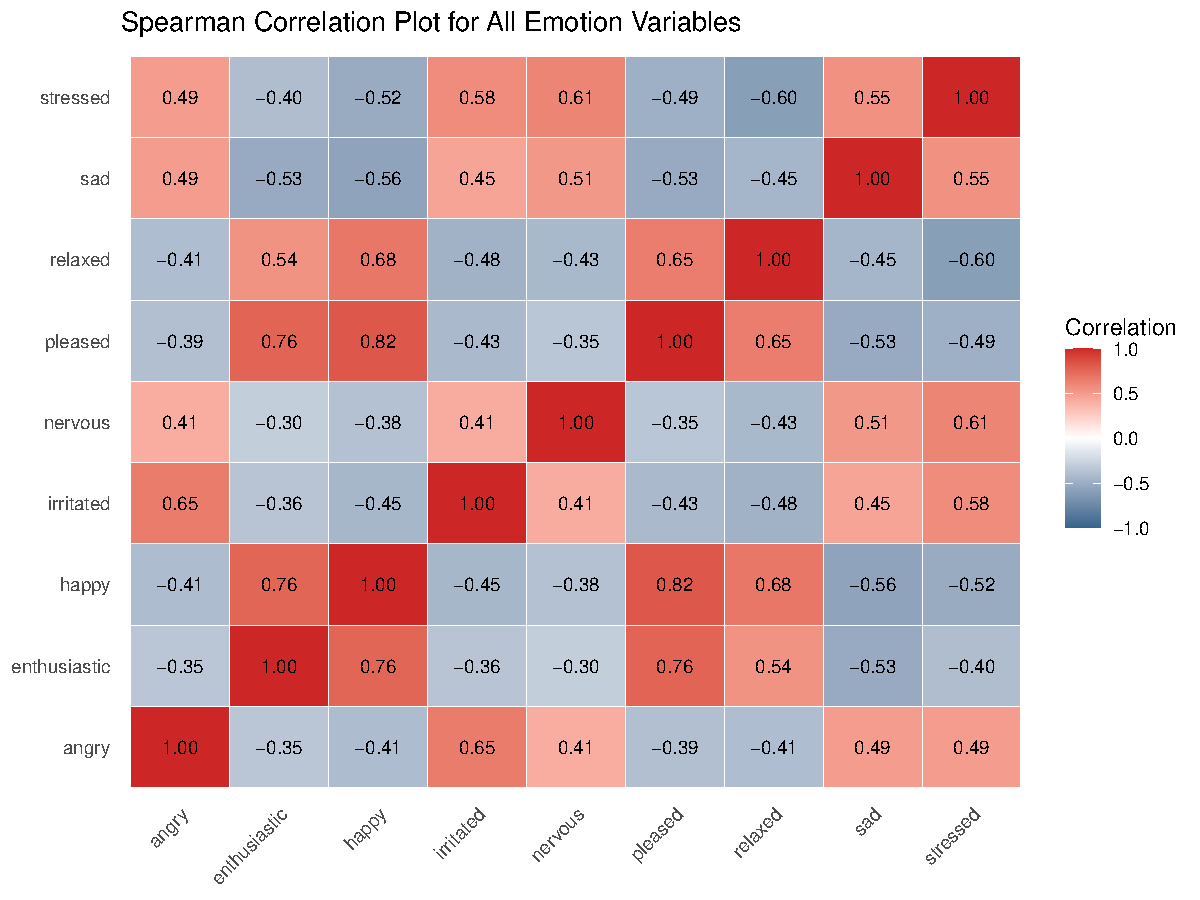
\includegraphics[width=0.8\textwidth]{corr_heatmap.pdf}
    \caption{Spearman correlation heatmap for the nine emotion variables.}
    \label{fig:corr_heatmap}
\end{figure}

To rank the candidate emotions by predictive usefulness, we carried out a leave-one-subject-out one-step-ahead prediction analysis. For each ordered predictor--target pair $(j,k)$ with $j \neq k$, we compared a baseline model and an augmented model:
\begin{align}
\text{Baseline model:}\qquad
Y_{i,t+1}^{(k)} &= \alpha_k + \beta_k Y_{i,t}^{(k)} + \varepsilon_{i,t}^{(k)}, \\
\text{Augmented model:}\qquad
Y_{i,t+1}^{(k)} &= \alpha_k + \beta_k Y_{i,t}^{(k)} + \gamma_{jk} Y_{i,t}^{(j)} + \varepsilon_{i,t}^{(k)}.
\end{align}
Here, the baseline model predicts the next value of target emotion $k$ using only its own lagged value, while the augmented model additionally includes predictor emotion $j$ at the previous time point. Thus, the augmented model tests whether emotion $j$ provides incremental predictive information beyond the target emotion's own temporal dependence.

Prediction performance was evaluated using leave-one-subject-out cross-validation. In each fold, one subject was held out as the test set, the models were fitted on the remaining subjects, and prediction error was computed on the held-out subject. This was repeated for every subject and then aggregated.

For each predictor emotion $j$, we summarized its overall predictive usefulness across all other target emotions by
\begin{equation}
\mathrm{Score}(j)
=
\frac{1}{K-1}
\sum_{k \ne j}
\frac{\mathrm{MSE}_{\text{baseline},k}-\mathrm{MSE}_{\text{augmented},k}}
{\mathrm{MSE}_{\text{baseline},k}},
\end{equation}
where $K=9$ is the number of emotions. This score is the mean relative reduction in out-of-sample mean squared error across all other target emotions. Larger values indicate stronger average incremental predictive value.

Table~\ref{tab:overall_scores} reports the resulting summary statistics. The column \texttt{total\_rmse\_gain} is the total reduction in RMSE across all target emotions, and \texttt{mean\_rmse\_gain} is the corresponding average reduction. The primary ranking criterion is \texttt{mean\_rel\_mse\_reduction}, which corresponds directly to the score above. Under this criterion, \texttt{happy} ranked first, indicating that it provided the largest average out-of-sample improvement when added as a lagged predictor for the remaining emotions. The column \texttt{median\_rel\_mse\_reduction} gives a more robust summary across targets and also placed \texttt{happy} first.

\begin{table}[htbp]
\centering
\scriptsize
\caption{Overall predictive screening scores from leave-one-subject-out cross-validation. Emotions were ranked primarily by mean relative MSE reduction.}
\label{tab:overall_scores}
\begin{tabular}{lrrrr}
\hline
Predictor & Total RMSE Gain & Mean RMSE Gain & Mean Relative MSE Reduction & Median Relative MSE Reduction \\
\hline
happy        & 0.026735 & 0.003342 & 0.005293 & 0.004320 \\
enthusiastic & 0.017941 & 0.002243 & 0.003581 & 0.003008 \\
relaxed      & 0.015705 & 0.001963 & 0.003187 & 0.003463 \\
pleased      & 0.012549 & 0.001568 & 0.002535 & 0.002532 \\
nervous      & 0.010544 & 0.001318 & 0.002081 & 0.001074 \\
stressed     & 0.008082 & 0.001010 & 0.001651 & 0.001179 \\
sad          & 0.007534 & 0.000942 & 0.001546 & 0.001556 \\
irritated    & 0.001180 & 0.000147 & 0.000307 & -0.000136 \\
angry        & -0.003500 & -0.000438 & -0.000716 & -0.000738 \\
\hline
\end{tabular}
\end{table}


\subsection{Forward Selection for Additional Predictors of \texttt{happy}}
\label{app:forward_selection_happy}

We used a forward-selection procedure to identify additional emotion variables that help predict future \texttt{happy}. At each step, we started from a baseline model containing \(\texttt{happy}_{i,t}\), then added one candidate emotion at time \(t\), and selected the candidate that gave the largest improvement in one-step-ahead prediction of \(\texttt{happy}_{i,t+1}\).

Prediction performance was evaluated using leave-one-subject-out cross-validation. In each fold, one subject was held out as the test set, the model was fitted on the remaining subjects, and prediction error was computed on the held-out subject. Candidates were ranked by their relative reduction in out-of-sample mean squared error,
\[
\frac{\mathrm{MSE}_{\text{base}}-\mathrm{MSE}_{\text{aug}}}{\mathrm{MSE}_{\text{base}}},
\]
where larger values indicate stronger incremental predictive value.

Table~\ref{tab:forward_selection_happy} shows the selected predictors at each step. The first three selected variables were \texttt{enthusiastic}, \texttt{relaxed}, and \texttt{pleased}. The predictive gain was largest at the first step and became smaller afterwards, suggesting diminishing additional benefit as more closely related positive emotions were added.

\begin{table}[htbp]
\scriptsize
\centering
\caption{Forward-selection results for predicting future \texttt{happy}.}
\label{tab:forward_selection_happy}
\begin{tabular}{r l r r r r r l}
\hline
Step & Candidate & RMSE Base & RMSE Aug & RMSE Gain & Relative MSE Reduction & \(n_{\text{obs}}\) & Selected So Far \\
\hline
1 & enthusiastic & 1.165833 & 1.161850 & 0.003984 & 0.006822 & 5941 & enthusiastic \\
2 & relaxed      & 1.161850 & 1.160139 & 0.001711 & 0.002943 & 5941 & enthusiastic, relaxed \\
3 & pleased      & 1.160221 & 1.159928 & 0.000293 & 0.000505 & 5940 & enthusiastic, relaxed, pleased \\
\hline
\end{tabular}
\end{table}
\subsection{Implentation R codes}

\printbibliography

\end{document}